\subsection{Esquema organizativo}

La organización del proyecto se articula en torno al comité dirección y al equipo de trabajo que se va a encargar de desarrollar el producto, en función de la estructura de la figura \ref{fig:org_schema}.

\begin{figure}[!htp]
	\centering
	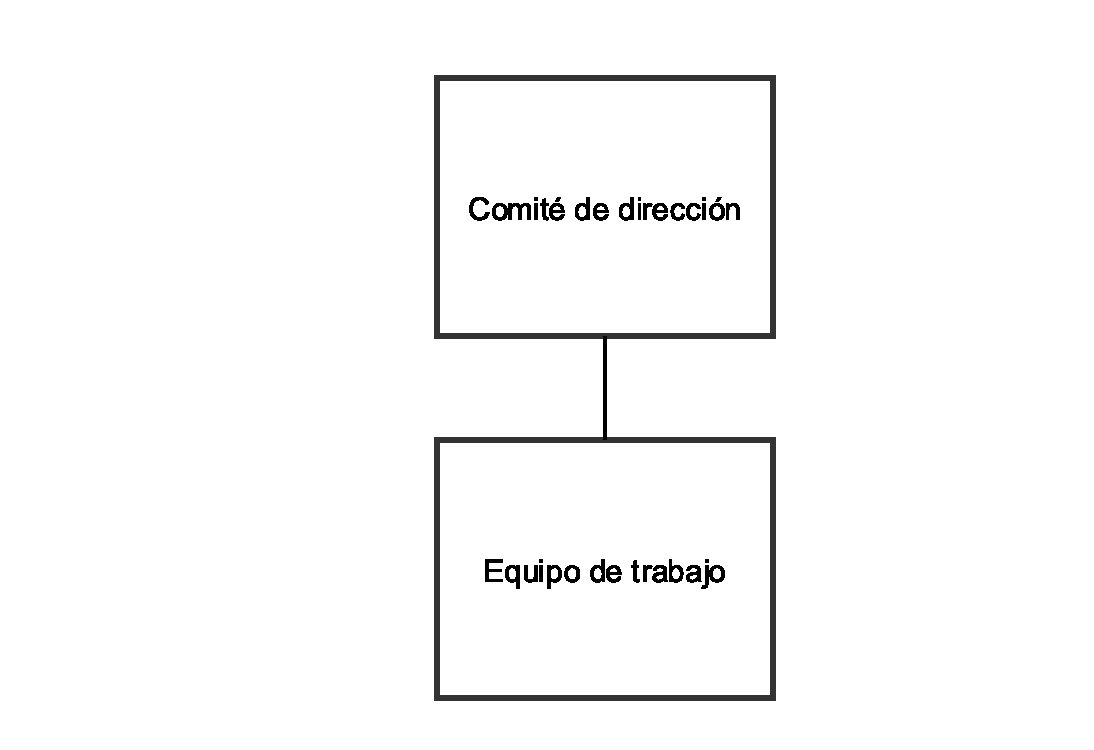
\includegraphics[scale=.75]{fig/organization}
	\caption{Esquema organizativo}\label{fig:org_schema}
\end{figure}

\begin{itemize}
	\item \textbf{Comité de dirección:} su función principal es orientar por dónde debería ir el proyecto y tomar las decisiones finales a la hora de qué hacer o no. Además, este comité deberá aprobar las diferentes fases del proyecto.
	\item \textbf{Equipo de trabajo:} el órgano encargado de diseñar y desarrollar el contenido del proyecto en función de las diferentes fases estipuladas.
	\item \textbf{Seguimiento:} Debido a el bajo número de personas que compone el equipo de desarrollo se ha acordado trabajar mediante reuniones de seguimiento semanales pero también tras terminar cada tarea. En las reuniones semanales se reunirán todos los miembros del equipo, mientras que en las que corresponden a una tarea finalizada lo harán solo los que han participado en dicha tarea junto a el director de proyecto. Su finalidad será comentar los avances y/o problemas que hayan podido ocurrir, aunque también servirán para que el director de el visto bueno a la tarea y pasar a la siguiente. 
\end{itemize}